\chapter[Proposta de Trabalho]{Proposta de Trabalho}


A proposta de trabalho consiste no desenvolvimento de uma aplicação descentralizada(dApp) para o registro de infrações de trânsito utilizando-se da tecnologia \textit{blockchain} para garantir a integridade das informações registradas. 

Será implementado um blockchain do tipo público, onde todos podem contribuir para o processo de consenso e validação dos blocos adicionados, possibilitando que qualquer pessoa interessada possa contribuir para a rede de registros. Para mais informações em relação a este tipo de blockchain, veja a seção \ref{subsection_tipos_blockchain}

Para auxiliar nos testes e uso da aplicação descentralizada durante o desenvolvimento, também serão utilizadas duas outras ferramentas: Ganache - Truffle Framework e o Metamask. O Ganache permite ativar e gerenciar rapidamente um blockchain pessoal Ethereum para executar testes, executar comandos e inspecionar o estado do mesmo enquanto controla como a cadeia de blocos opera. O Metamask é um plug-in adicionado ao navegador, que serve como uma ponte para conectar-se à rede e injetar a instância web3 em no código. O Metamask também permite selecionar redes diferentes (como uma local para testes) e contas Ethereum.
Mais informações sobre a execução e instalação dessas ferramentas estão disponíveis nos apêndices X e Y.


\section{Aplicação}

O dApp(aplicação descentralizada) será criado para tornar o registro infrações de trânsito transparentes e descentralizados. Angular será usado para implementar o \textit{front-end} e os contratos inteligentes solidity da plataforma ethereum serão usados no \textit{back-end}. 

Angular é uma estrutura JavaScript usada para criar aplicativos de página única. A principal característica é que podemos criar nossos aplicativos de maneira modular, o que ajuda a reduzir a repetição de códigos e facilita a depuração. Ele também permite modificar os elementos HTML dinamicamente, facilitando a criação de páginas interativas em tempo real. 

Os contratos inteligentes escritos em solidity para a rede ethereum no back-end da aplicação torna o dApp descentralizado e transparente. 

\subsection{Arquitetura Proposta}

A arquitetura da aplicação será no estilo cliente servidor. O dApp conterá duas partes principais: o contrato, sendo executado na rede ethereum, e o aplicativo cliente sendo executado localmente no computador do usuário.

Exemplo da comunicação:

    \begin{figure}[H]
         \centering
         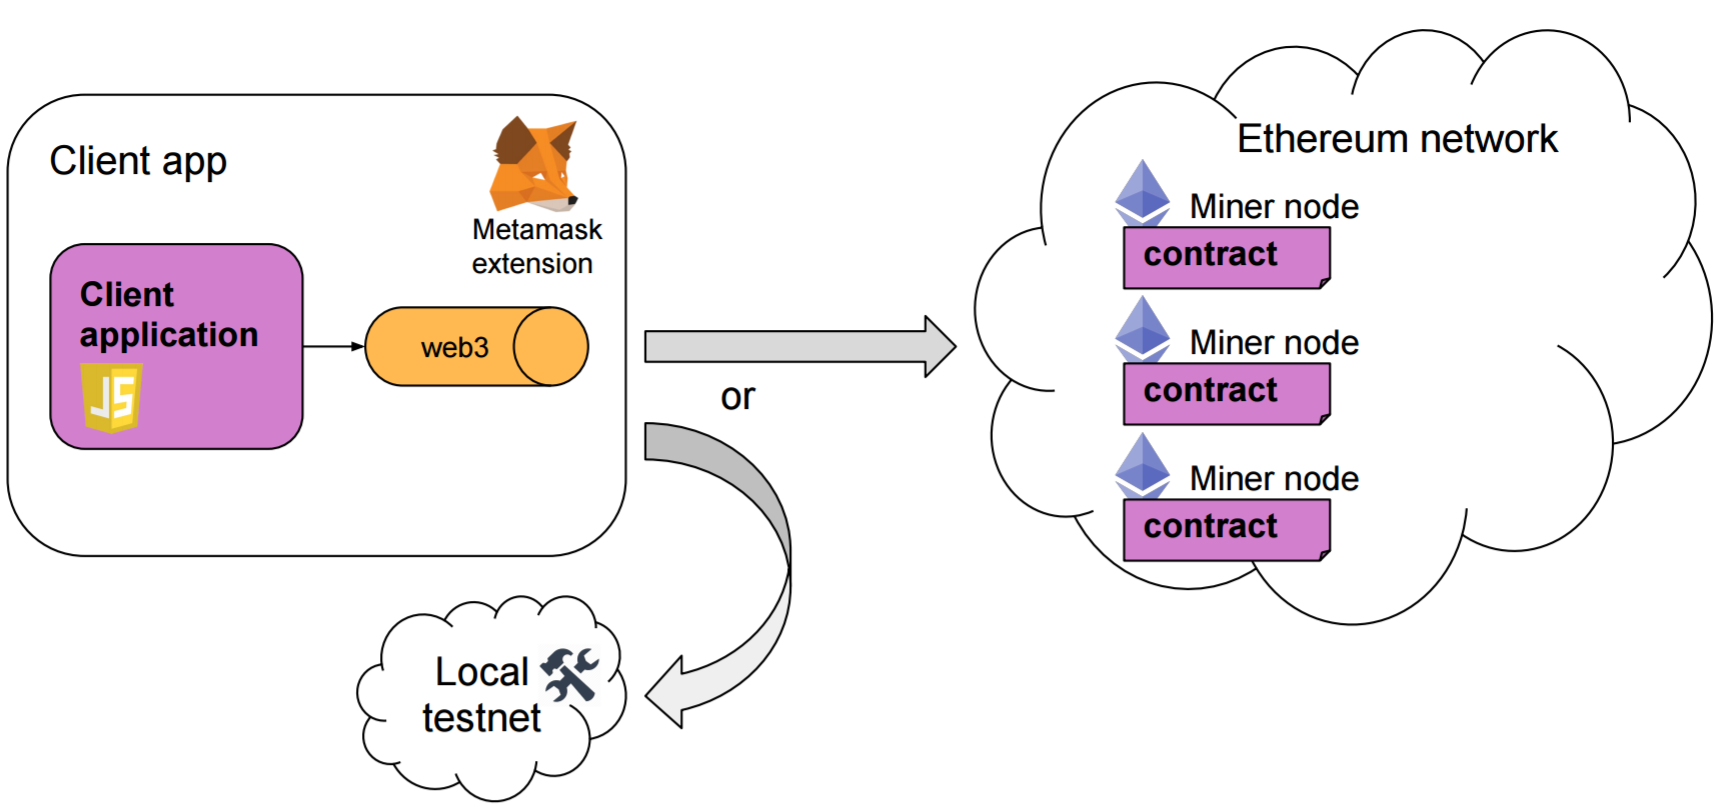
\includegraphics[scale=0.25]{figuras/capitulo_3/dapp_representacao_comunicacao.png}
         \caption{Representação das partes - Imagem retirada de \href{https://sites.google.com/site/blockchaintutorial/dapp-architecture}{DApp Architecture}}
         \label{fig:dapp_representacao}
    \end{figure}



\subsection{Funcionalidades}

O DApp contemplará as seguintes funcionalidades:


    \subsubsection{Registro de Infração}
    
        Aqui, a autoridade governamental registrada como administrador registra as informações relacionadas ao registro de infração. O administrador verifica os detalhes com os registros existentes e entra no dApp. As informações que serão cadastrados no dApp para o registro da infração são:
        
        \begin{itemize}
            \item Placa do veículo
            \item Categoria da Infração
            \item Data/Hora da Infração
            \item Pontos da Infração
            \item Observações
            \item Administrador responsável pela aplicação
            \item Preço para pagamento da infração (valor em ethers)
            \item Data limite para pagamento
        \end{itemize}
    
        Junto com essas informações, um ID gerado a partir dos quatro primeiros campos também é inserido. Este ID será gerado em uma função usando SHA256. Os valores inseridos no formulário serão passados para a função de registro e os detalhes são mapeados usando o ID gerado acima. Mais tarde, esse mapeamento permite a busca de um registro ser realizada mais facilmente.
        
        Após confirmar as informações preenchidas, a transação será inserida no blockchain e validada por outros nós. Após este processo a infração estará disponível para que sejam realizadas as outras funções como consulta, realização de recursos e pagamento da mesma.
        
            
    \subsubsection{Transferência de Infração}
    
        Nesta funcionalidade, o usuário indicado como autor da infração registrada poderá transferir para outro usuário a autoria da infração de trânsito.
        
        Ao visualizar as informações da infração, o usuário(A) terá uma opção disponível para inserir a chave de outro usuário(B), e realizar a indicação de autoria. Este usuário(B) terá em sua página uma indicação dessa solicitação e terá disponível as opções: aceitar ou recusar. Caso o usuário(B) aceite a transferência assinando a transação com sua chave, a transação indicando a transferência será realizada de forma automática sem a necessidade da interferência de um usuário administrador(C).
    
    \subsubsection{Busca de Infrações}
    
        A busca de infrações consistirá em dois módulos diferentes: busca realizada pelo administrador e busca do usuário normal.
        
        O usuário registrado como administrador poderá consultar os registros de diferentes formas, como: infrações de um usuário específico, ou por um veículo.
        
        Já o usuário normal terá em sua página de acesso todas as infrações que foram registradas como ele sendo o autor da infração, não sendo possível visualizar as infrações realizadas por outros usuários.
    
    \subsubsection{Pagar Infração}
    
        O pagamento da infração poderá ser realizada pelo usuário indicado como responsável pela infração. Para este pagamento serão utilizadas as moedas virtuais da rede ethereum, de acordo com o valor indicado na infração acrescido das taxas necessárias para a realização da transação.O pagamento de uma infração corresponde à ação de transferir os valores referentes ao pagamento da infração para a conta da união registrada na rede blockchain.
    
    
    \subsubsection{Recurso / Cancelamento de uma infração}
    
        Ao visualizar a infração o usuário(A) indicado como responsável também poderá entrar com recurso em relação a infração registrada. Esta condição se aplica a casos onde o usuário não concorda com a infração registrada ou possui uma explicação plausível que pode acarretar na anulação da mesma.
        
        Para realizar esta ação o usuário(A) deverá clicar na opção disponível, preencher as informações solicitadas e assinar a solicitação usando sua chave. Essa solicitação irá para análise por parte de um usuário(B) administrador, e o mesmo poderá recusar ou aceitar a solicitação realizada.
        
        Caso o usuário(B) administrador aceite o recurso realizado, uma transação será inserida no blockchain anulando a infração registrada anteriormente e removendo a responsabilidade do usuário(A) em relação a mesma.
        
        
\subsection{Minerar moedas}

Para minerar moedas ethereum é necessário ter um computador com alta capacidade de processamento. O papel destes mineradores é encontrar uma sequência que torne um bloco de transações compatível com o bloco anterior. Para isso, o computador precisa efetuar milhares de cálculos por segundo para encontrar a combinação perfeita, por isso que eles precisam ser extremamente potentes.

Ao encontrar a sequência compatível, o minerador recebe uma recompensa para cada bloco que ele minerar. Essa recompensa foi criada com a intenção de pagar as pessoas que emprestam poder computacional para manter a rede funcionando.

De forma a incentivar a inserção do maior número de nós possíveis na rede, tornando a confiabilidade da rede ainda maior, o pagamento das infrações registradas no blockchain poderão ser feitas utilizando essas moedas obtidas por meio da mineração. Este incentivo beneficiará principalmente pessoas jurídicas que possuem uma grande frota automotora e serviços computacionais a disposição, como empresas locadoras de veículos e empresas de transporte urbano, pois eles poderão pagar as infrações realizadas por sua frota com um certo desconto e ainda beneficiarão a rede como um todo.
